\documentclass[conference]{IEEEtran}
\IEEEoverridecommandlockouts
\usepackage{cite}
\usepackage{amsmath,amssymb}
\usepackage{graphicx}
\usepackage{booktabs}
\usepackage{url}
\usepackage{array}
\hyphenation{cy-ber-se-cur-i-ty cryp-to-graph-ic}

\begin{document}

\title{Implementation and Functional Evaluation of an Educational Secure-Messaging and Security-Analysis Laboratory}

\author{\IEEEauthorblockN{[Author Name]}
\IEEEauthorblockA{[Department and Institution]\\
[City, Country]\\
[Email address]}}

\maketitle

\begin{abstract}
This paper presents the design and functional evaluation of CNS Security Lab, a controlled web application for teaching message confidentiality and integrity, manual relay interception, malware scanning, and bounded website analysis. A Flask service hosted by Ubuntu stores SQLite records and cryptographic keys; Windows and Kali Linux virtual machines act as browser clients on a host-only network. Protected application messages are encrypted with AES-256-GCM under a server-held instance master key and signed with per-user Ed25519 keys. The optional browser transport exercise uses finite-field ElGamal-style key transport and AES-GCM, but terminates at the server and is not end-to-end encryption. The dependency-complete pytest run collected 114 cases: 113 passed, one platform-specific permission test was skipped, and none failed. A separate local microbenchmark measured 100 trials per condition for 16-, 256-, 1024-, and 2000-byte inputs using the actual envelope routines and an AES-GCM-only primitive baseline. At 1024 bytes, median encrypt/sign was 50.05 microseconds versus 1.20 microseconds for AES-GCM-only; median verify/decrypt was 95.15 versus 1.20 microseconds. These are local microbenchmark comparisons, not HTTP latency or a causal estimate of security overhead. We detail the implementation, threat model, measured data, reproducible methods, and limitations.
\end{abstract}

\begin{IEEEkeywords}
authenticated encryption, cybersecurity education, digital signatures, Flask, secure messaging, security testing
\end{IEEEkeywords}

\section{Introduction}
Secure-message demonstrations are most informative when they distinguish confidentiality, integrity, endpoint authentication, and trust in the server. CNS Security Lab combines a messaging application with an application-scoped manual relay, bounded file and website analysis, and persistent audit and scan records. The relay allows an authorized operator to forward, alter, or drop messages submitted through the intentionally unprotected path. This is a controlled teaching simulation; it does not capture general network traffic or provide an independent attacker host.

This study asks: (RQ1) do the implemented envelope-verification paths reject the tested ciphertext, signature, nonce, and metadata changes? (RQ2) do tested message-ownership and identifier-enumeration requests prevent a nonparticipant from reading protected messages? (RQ3) do the tested mutation routes enforce CSRF and session revocation behavior? (RQ4) what is the local cost of the complete envelope functions relative to the AES-GCM primitive for supported message sizes? We hypothesize that the specific negative cases asserted by the regression suite are rejected (H1--H3) and that the complete envelope functions have higher median time than the primitive-only baseline (H4). We do not hypothesize detection accuracy or request-latency improvement because no labeled scanner corpus or HTTP-level timing instrumentation is present.

The contributions are an implementation-level trace of the application, formal notation for the actual cryptographic envelope, a threat and limitation analysis, and a reproducible evaluation of the current automated test suite. Our evidence is intentionally separated from security claims: a passing test means a program assertion succeeded under its harness, not that a real attacker is blocked under all conditions.

\section{Related Work}
Formal analyses of the Signal protocol model authenticated key agreement and ratcheting properties that a secure messaging design may seek to provide \cite{cohn2017signal}. CNS Security Lab does not implement a ratchet, asynchronous key agreement, forward secrecy, post-compromise security, or recipient-held end-to-end keys. It instead provides a deliberately simpler, server-decryptable envelope so message alterations can be inspected in a classroom.

Black-box web vulnerability scanners have been evaluated against vulnerable applications and representative bug classes; prior work emphasizes that scanners can miss vulnerabilities and report spurious findings \cite{doupe2010}. This motivates treating the lab's bounded response heuristics as evidence collection rather than a general vulnerability verdict. OWASP's Web Security Testing Guide likewise frames testing as a selected, scoped methodology and not a proof of absence \cite{owaspwstg}. We use NIST's GCM specification, RFC 8032, RFC 3526, and official implementation documentation to describe primitives and API behavior \cite{nistgcm,rfc8032,rfc3526,pyca}.

\section{Architecture and Threat Model}
\subsection{Deployment and components}
The reference VirtualBox topology places Flask, SQLite, ClamAV, the key directory, and the administrator relay view on Ubuntu (example address 192.168.56.102). Windows (192.168.56.1) and Kali (192.168.56.101) are browser clients over a host-only network. All addresses are runbook examples, not verified addresses from the evaluation run. The application is configured for HTTPS on port 5000 in the VM scenario. The generated certificate is trusted on client VMs; the private key remains on Ubuntu. Live VM routing, TLS trust, and ClamAV timing were not tested in this evaluation. Flask's built-in development server is not an appropriate production WSGI deployment \cite{flaskdeploy}.

The implementation uses Python, Flask, Flask-SQLAlchemy/SQLAlchemy, Flask-Login, Flask-WTF, and PyCA cryptography. Jinja renders pages; ordinary JavaScript and CSS implement client interactions; ReportLab generates PDF scan reports; SQLite persists accounts, messages, relay items, events, scans, and findings. ClamAV is an external Ubuntu command-line scanner. This application does not use a React frontend. The principal request path is browser form or JSON request $\rightarrow$ route authentication/validation/CSRF $\rightarrow$ service operation $\rightarrow$ ORM/database and key store $\rightarrow$ JSON, rendered page, or file response.

\subsection{Assets, trust, and adversary}
Assets include plaintext message content, account credentials and sessions, signing private keys, the instance master key, uploaded files, scan targets/results, and audit data. The server process and Ubuntu operator are inside the trusted computing base: the server holds the AES master key and can decrypt stored messages. External URLs, uploaded bytes, browser requests, and relay operations are treated as untrusted input. The educational relay operator is an authenticated administrator, not an arbitrary network adversary.

The considered attacks include modification of ciphertext/signature/nonce/metadata, unauthorized message reads and numeric ID sweeps, forged cross-site mutations, repeated login attempts, unsafe external-target resolution/redirects, and malformed or oversized uploads. Automated tests exercise selected cases. Denial of service, hypervisor compromise, host compromise, browser compromise, distributed credential attacks, real-world malware detection rates, and complete web vulnerability coverage are outside measured scope. IDOR findings in tests establish only the specific owner-scoped routes and fixtures exercised.

\section{Cryptographic and Mathematical Model}
\subsection{At-rest message envelope}
The source uses one 32-byte instance master key $K_M$ for AES-GCM message encryption and key wrapping. It does not derive a distinct key per message. For plaintext $P$, fresh 96-bit nonce $N$, and canonical associated data $A$ containing version, UUID, sender/recipient identifiers, timestamp, and algorithm, encryption is
\begin{equation}
(C,T)=\operatorname{GCM.Enc}_{K_M}(N,P,A),
\label{eq:gcm}
\end{equation}
where $C$ is the ciphertext and $T$ is the authentication tag (the PyCA AESGCM byte string contains ciphertext and tag). AES-GCM is an authenticated-encryption-with-associated-data mode \cite{nistgcm,pyca}. The implementation uses the metadata JSON as AAD and a random 12-byte nonce. Nonce uniqueness under a given key is a critical operational requirement; the code uses random nonces but does not maintain a separate deterministic counter or formal per-key collision budget.

The signed input is domain separated and binds canonical metadata, nonce, and the ciphertext byte string (including the GCM tag):
\begin{equation}
\begin{aligned}
\sigma=\operatorname{Ed25519.Sign}_{sk_s}(&D\parallel J(A,N)\parallel\texttt{LF}\\
&\parallel(C\parallel T)),
\end{aligned}
\label{eq:sign}
\end{equation}
where $sk_s$ is the sender signing key, $D$ is the fixed protocol label, and $J$ is sorted, compact ASCII JSON. The receiver verifies the sender's Ed25519 public key first and releases plaintext only if signature verification and GCM authentication both succeed:
\begin{equation}
\begin{aligned}
\operatorname{Accept}(P)\iff{}&\operatorname{Verify}_{pk_s}(\sigma,m)=1\\
&{}\land\operatorname{GCM.Dec}_{K_M}(N,C\parallel T,A)=P.
\end{aligned}
\label{eq:accept}
\end{equation}
Ed25519 signatures are specified by RFC 8032 \cite{rfc8032}. Public keys are associated with account rows; the implementation does not provide an external key-transparency mechanism or independently verified identity channel. AEAD integrity and signature authenticity are therefore conditional on key protection and account/key binding.

Per-user Ed25519 private keys are AES-GCM-wrapped with the same instance master key, fresh wrapping nonce, and AAD \texttt{cns-user-key:<uid>}. POSIX key-directory/file modes are restricted to owner access. A missing key for an extant database causes a hard error rather than silent key regeneration. Because $K_M$ is shared by message ciphertexts and wrapped signing keys, compromise of the master key exposes both classes of data. Key separation, master-key rotation, and a dedicated secret-management boundary are not implemented.

\subsection{Browser transport teaching exercise}
When both accounts enable browser protection, the browser JavaScript encrypts the submission using an AES-GCM key represented by integer $m$ and transports that key using a finite-field ElGamal-style operation. The service uses RFC 3526 Group 5's 1536-bit prime $p$ and generator $g=2$ \cite{rfc3526}. The server holds secret exponent $x$ and publishes $y=g^x\bmod p$. The client selects ephemeral $k$, computes $c_1=g^k\bmod p$ and $c_2=m y^k\bmod p$. The server obtains
\begin{equation}
s=c_1^x\bmod p,\qquad m=c_2s^{-1}\bmod p.
\label{eq:elgamal}
\end{equation}
The recovered value is converted to 32 bytes and used as an AES-256-GCM key; transport AAD includes a version label and normalized recipient. The application then processes its ordinary signed envelope. This construction is a teaching mechanism and is not a reviewed KEM: the finite-field size is legacy, the server holds the decryption exponent, and there is no KDF. Thus it does not provide end-to-end encryption or forward secrecy. The VM deployment's HTTPS listener protects the network channel only to the Ubuntu TLS endpoint.

\subsection{Hash and score definitions}
For file bytes $F$, the scanner computes $h=\operatorname{SHA256}(F)$ in a streaming pass. The SHA family is specified by NIST FIPS 180-4 \cite{fips180}. The web scanner's score is a transparent maximum-severity rubric, not CVSS. For finding set $\mathcal{F}$, $w$ maps Critical/High/Medium/Low/Informational to $100/75/50/25/0$:
\begin{equation}
R(\mathcal{F})=\begin{cases}0,&\mathcal{F}=\emptyset,\\\max_{f\in\mathcal{F}}w(\operatorname{severity}(f)),&\text{otherwise.}\end{cases}
\label{eq:risk}
\end{equation}
Confidence is separate from severity; failed or timed-out scans have no score.

\section{Implementation and Evaluation Method}
\subsection{Message and relay flow}
For protected messaging, services.crypto encrypts with the instance master key, signs the envelope using the sender's Ed25519 key, and persists nonce/ciphertext/signature and metadata. On read, the route scopes the message to sender or recipient; messaging.open\_message verifies the signature before decryption, and returns no plaintext on signature/tag failure. The signed metadata covers sender, recipient, timestamp, message UUID, version, algorithm, and nonce.

For the lab relay, compose forms place submitted plaintext in an application-scoped interception record. A protected transport request is used when both account settings permit it; a mixed protected/unprotected state is rejected rather than silently downgraded. An administrator may drop, forward the unchanged body, or forward an edited body. Forwarding unchanged preserves the original signature; edited content is re-encrypted but the original signature is retained, so the signature check fails. This provides a deterministic tamper demonstration but the operator is authorized and the server itself can read the plaintext relay item.

\subsection{Authentication and authorization}
Passwords are processed with Werkzeug's password-hash API; the login route uses a dummy hash for an unknown username, generic invalid-credential text, per-user/IP and per-IP attempt throttles, and server-tracked sessions. Session IDs are stored as SHA-256 digests; revocation and a password-change epoch invalidate sessions. Cookies are HttpOnly and SameSite=Lax and become Secure when HTTPS is configured. Flask-WTF tokens protect form and JSON mutations, with JavaScript sending X-CSRFToken. These controls follow common synchronizer-token and cookie-hardening patterns; OWASP also emphasizes testing CSRF defenses in the context of authenticated browser requests \cite{owaspcsrf}.

\subsection{File and website analysis}
File scanning enforces extension/type checks, a default 10-MiB limit, streaming 64-KiB reads, SHA-256, and a private temporary path. ClamAV is invoked with an argument vector and shell disabled; a timeout and a two-process semaphore bound execution. Only a completed clean result is treated as clean; detection, absence, errors, timeout, or busy status are non-clean. ClamAV documents the distinctions between its scan tooling and database updates; the application calls the one-shot clamscan executable rather than a persistent daemon interface \cite{clamav}. The scanner does not unpack archives or claim complete content-disarm.

The streaming hash processes an $n$-byte file in chunks of $q=65{,}536$ bytes, so application buffering is $O(q)$ and hash work is $O(n)$. For a comprehensive website scan, the root fetch permits at most $r=4$ redirects and each of $p=5$ fixed probes permits none. With per-root-response cap $B=262{,}144$ bytes and probe cap $Q=2{,}048$ bytes, a conservative request/body bound is
\begin{equation}
\begin{aligned}
N_{req}&\leq 1+r+p=10,\\
B_{total}&\leq B+pQ=272{,}384\;\mathrm{bytes}.
\end{aligned}
\label{eq:scanbound}
\end{equation}
The redirect chain shares the root fetch's cumulative body budget; the five fixed probes each have a 2-KiB budget and no redirect allowance. These application-level caps do not include protocol headers or resolver memory/time. DNS resolution can block beyond the nominal job deadline, so wall-clock duration is best-effort rather than a hard bound.

URL scanning accepts HTTP(S) on ports 80/443, rejects embedded credentials/control characters/local names/non-global IPs, resolves all addresses and rejects the target if any address is non-global, and connects to a validated address. HTTPS uses the normal certificate and hostname checks. Redirect destinations are revalidated, remain on the original host, and are limited to four. Each response body is capped at 256 KiB; URL length is capped at 2048 characters. Comprehensive mode checks five fixed same-host paths, while quick mode fetches the origin only. No JavaScript execution, crawling, authentication, brute force, or exploit payload is performed. SSRF defenses require complementary egress controls and careful redirect/DNS handling; OWASP describes layered mitigations \cite{owaspssrf}.

\subsection{Test protocol and evidence}
From the project root with its Python virtual environment, we executed \texttt{python -m pytest -q --tb=short --junitxml=docs/pytest-results-current.xml --basetemp=docs/pytest-tmp-current} on Windows 11 (reported host name Iffat), Python 3.14.7, pytest 9.1.1, Flask 3.1.3, Flask-SQLAlchemy 3.1.1, SQLAlchemy 2.1.4, and cryptography 50.0.2. ReportLab 4.5.1 was installed from the declared requirements after the initial run exposed that it was missing; the first run's PDF-export case returned 503, and the dependency-complete rerun succeeded. The final JUnit report records 114 parametrized test cases, 113 passed, one skipped, zero failed, and 108.395 seconds suite time. The skipped case checks POSIX-only file permissions, unavailable on Windows.

The test harness uses isolated temporary databases and keys. It is not a live Ubuntu/Kali/Windows network experiment. The JUnit report records per-case elapsed time; these times include test setup, password hashing, application/database work, and fixture effects and must not be interpreted as message latency. \texttt{experimental\_data.csv} retains per-case outcomes and durations. The separately executed \texttt{benchmark\_crypto.py} measures \texttt{encrypt\_and\_sign} and \texttt{decrypt\_envelope} against AES-GCM-only operations at 16, 256, 1024, and 2000 UTF-8 bytes, with 100 trials for each operation/size/mode. Execution order is randomized within each trial. The AES-GCM baseline uses the same key, payload size, and associated data derived from a prepared envelope; it omits metadata creation, Ed25519 signing/verification, and request/database work. Timings use \texttt{perf\_counter\_ns}. \texttt{crypto\_benchmark.csv} contains each observation. The analysis script reports mean, median, sample standard deviation, nearest-rank 95th percentile, and percentile-bootstrap 95\% confidence intervals for the median (2000 deterministic resamples). These CIs describe this local sample under a bootstrap assumption; they are not system-level confidence intervals. Figures~\ref{fig:outcomes}--\ref{fig:crypto} are generated from raw CSV records. There are no ground-truth vulnerability labels, so precision, recall, F1, confusion matrices, scanner detection rates, and attack-blocking rates are not computed.

\begin{figure*}[t]
\centering
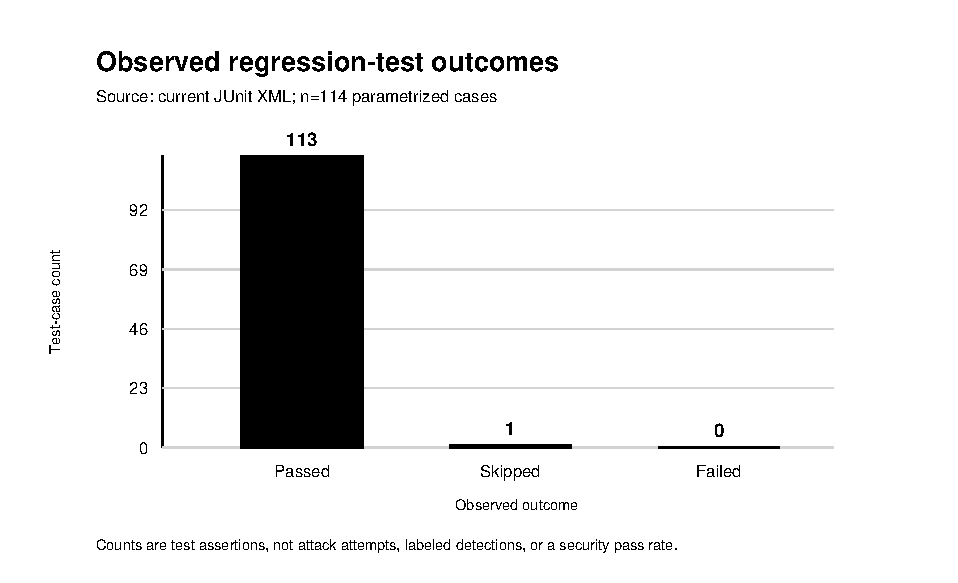
\includegraphics[width=\textwidth]{figures/test_outcomes.pdf}
\caption{Observed current pytest outcomes (114 test cases). Source: JUnit XML from the dependency-complete run; one test was skipped because the execution host was Windows. These are regression assertions, not a security detection-rate estimate.}
\label{fig:outcomes}
\end{figure*}

\begin{figure*}[t]
\centering
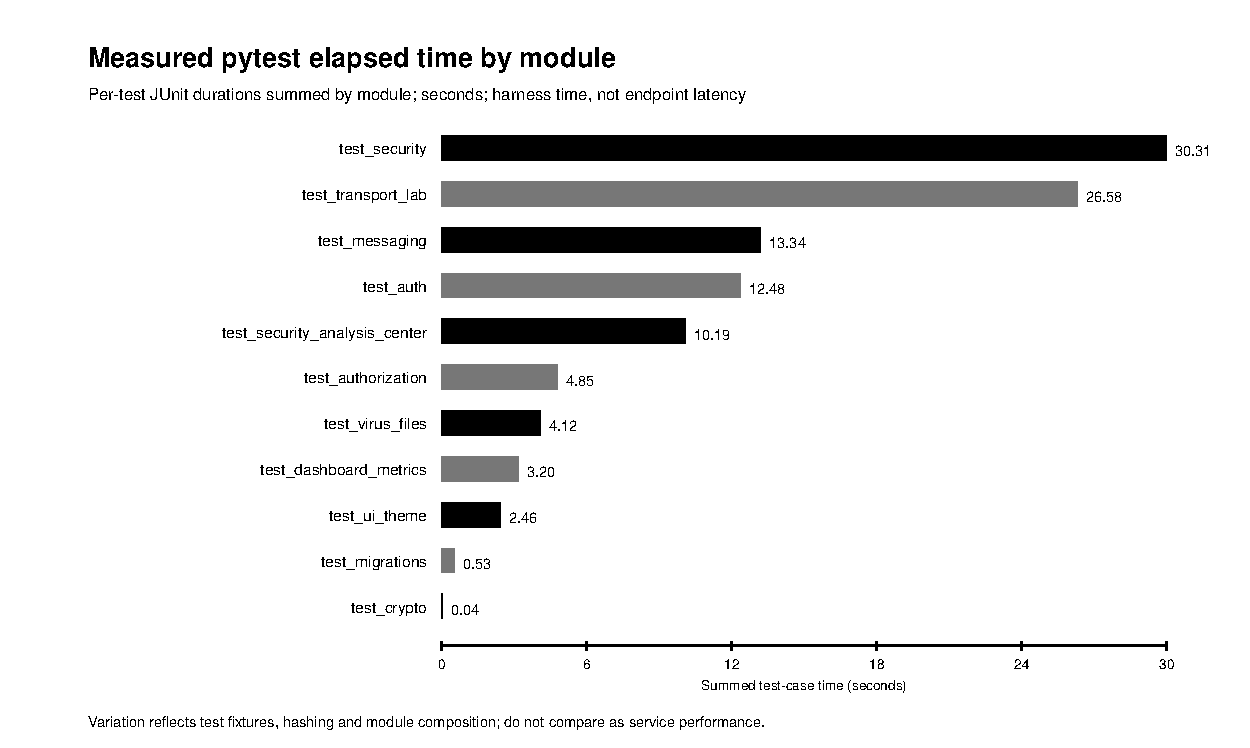
\includegraphics[width=\textwidth]{figures/test_runtime_by_module.pdf}
\caption{Sum of JUnit per-case elapsed time by test module, in seconds. Source: measured JUnit data ($n=114$). This is test-harness runtime, not a controlled service-latency benchmark.}
\label{fig:runtime}
\end{figure*}

\begin{figure*}[t]
\centering
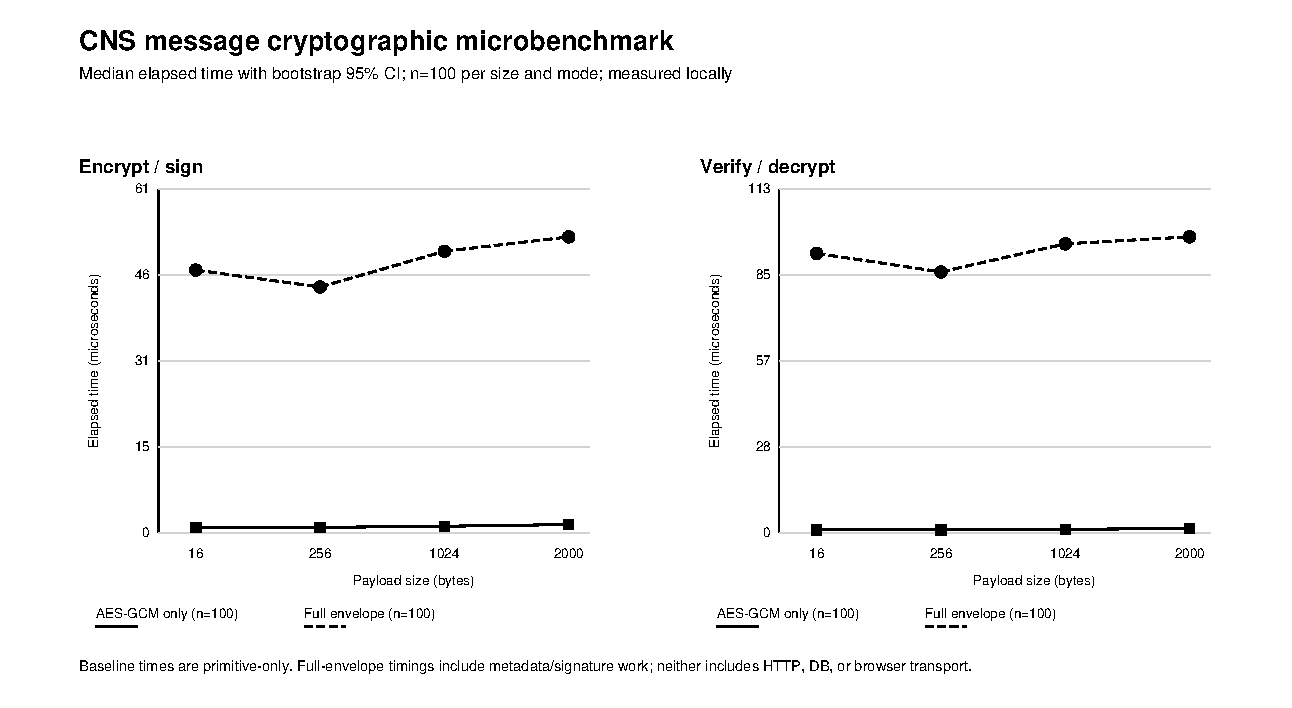
\includegraphics[width=\textwidth]{figures/crypto_overhead.pdf}
\caption{Measured median time and bootstrap 95\% confidence interval for the complete application envelope functions and the primitive-only AES-GCM baseline. Each point has $n=100$ trials. The comparison omits HTTP, persistence, TLS, and browser transport and is therefore a local function-level microbenchmark.}
\label{fig:crypto}
\end{figure*}

\section{Results and Discussion}
The final run's 113 passing assertions support H1--H3 only for the exact inputs and routes asserted by the repository tests. Cryptographic unit tests exercise round trip, nonce length/uniqueness across 500 generated test messages, ciphertext/signature/nonce mutation, metadata mutation, wrong sender key, invalid-signature verification before decryption, and a validly signed envelope opened with the wrong master key. Authorization tests assert that a third account receives 404 for selected message, envelope, and HTML routes and that an ID sweep yields only 404. CSRF and session tests cover selected missing/forged tokens and logout revocation. Relay tests verify selected delivery and tamper paths. The suite result does not establish cryptographic strength or all-route coverage.

The crypto microbenchmark supports H4 in this specific environment: at 1024 bytes, median full encrypt/sign was 50.05~$\mu$s (bootstrap 95\% CI 49.70--50.55~$\mu$s) versus 1.20~$\mu$s (1.20--1.30~$\mu$s) for AES-GCM-only. Median full verify/decrypt was 95.15~$\mu$s (94.55--96.00~$\mu$s), compared with 1.20~$\mu$s (1.10--1.30~$\mu$s) for AES-GCM-only. The full encryption routine includes timestamp/UUID/nonce generation, canonical metadata serialization, AES-GCM object work, and Ed25519 signing. The full decryption routine includes canonical metadata reconstruction, AESGCM object work, Ed25519 verification, and authenticated decryption. The baseline reuses an AESGCM object and precomputed AAD; for encryption it also pre-generates the nonce. Thus the observed gap is the cost difference between these measured functions, not isolated signature cost or HTTP-level security overhead. Fig.~\ref{fig:crypto} shows all four sizes. For $n$ measured durations $x_i$, the reported mean and sample standard deviation are
\begin{equation}
\begin{aligned}
\bar{x}&=\frac{1}{n}\sum_{i=1}^{n}x_i,\qquad
s=\sqrt{\frac{1}{n-1}\sum_{i=1}^{n}(x_i-\bar{x})^2},\\
P_{95}&=x_{(\lceil0.95n\rceil)}.
\end{aligned}
\label{eq:latency}
\end{equation}
Here $x_{(j)}$ is the $j$th sorted observation. Median confidence intervals are percentile intervals from 2000 bootstrap resamples of the 100 timing observations.

Figure~\ref{fig:runtime} reports module-level per-test elapsed sums from JUnit; expensive password-hash fixtures and test composition confound comparisons. No HTTP request-size latency sweep, concurrent-load test, throughput test, cross-platform comparison, or Ubuntu/ClamAV scan timing was performed. The one-machine microbenchmark is descriptive; its bootstrap intervals do not account for machine, OS, interpreter, or thermal variation.

Figure~\ref{fig:outcomes} reports 113 passed, one skipped, and zero failed in the dependency-complete run. The first run before ReportLab installation had one failed PDF-export test and one skipped platform permission test. After installing the declared ReportLab dependency, the suite passed 113 cases with that one skip. This illustrates why environment completeness is part of reproducibility. The skipped POSIX permission assertion remains unverified here and should be exercised on Ubuntu. ClamAV behavior and real web targets were not measured.

\section{Security Analysis and Limitations}
The current application server is a trusted party and a single point of compromise: it has the master key, decrypts messages, and wraps signing keys under that same key. The browser transport's ElGamal secret is also server-side. The lab therefore teaches authenticated encryption and signature verification, not a deployable end-to-end architecture. A server compromise exposes message plaintext and may expose per-user signing keys. Key separation and recipient-only decryption should be requirements for any successor.

The regression suite is not a penetration test. It does not prove that every API object is owner-scoped, that all CSRF routes are protected, or that a browser certificate is correctly trusted in every VM. It does not quantify URL-scanner false positives/negatives because the scanner has no labeled corpus. DNS resolver calls may exceed the nominal scan deadline; bounded application logic cannot replace network egress policy. ClamAV clean status is not a safety guarantee. Macro-enabled Office files are treated as suspicious for manual review even if the engine reports clean. The manual relay is app-scoped and cannot inspect unrelated traffic.

The score in (\ref{eq:risk}) is a prioritization rubric only. For a binary detector with defensible ground truth, define true positive (TP) as a vulnerable fixture correctly flagged, true negative (TN) as a benign fixture not flagged, false positive (FP) as a benign fixture flagged, and false negative (FN) as a vulnerable fixture missed. The standard metrics are
\begin{equation}
\begin{aligned}
\mathrm{Precision}&=\frac{TP}{TP+FP},\quad \mathrm{Recall}=\frac{TP}{TP+FN},\\
\mathrm{Accuracy}&=\frac{TP+TN}{TP+TN+FP+FN}.
\end{aligned}
\label{eq:metrics}
\end{equation}
\begin{equation}
\begin{aligned}
F_1&=2\frac{\mathrm{Precision}\cdot\mathrm{Recall}}{\mathrm{Precision}+\mathrm{Recall}},\\
R_{block}&=100\frac{N_{blocked}}{N_{attempted}}\%.
\end{aligned}
\label{eq:f1}
\end{equation}
A zero denominator makes the corresponding quantity undefined. $N_{blocked}$ and $N_{attempted}$ count explicit attack requests with observed outcomes, not test cases. No labeled scanner corpus or standalone attack-attempt dataset exists here; these metrics are not instantiated.

\section{Proposed Reproducible Experiments and Future Work}
Table~\ref{tab:experiments} distinguishes performed assertions from proposed measurements. Proposed work should use a local, disposable test deployment and controlled test users, not unrelated public sites. For a message-size benchmark, instrument client/server boundaries around encryption, signing, storage, reading, verification, and decryption; test sizes such as 16 B, 1 KiB, 16 KiB, and 256 KiB with at least 100 randomized trials per size and paired baseline/security configurations on the same host. Report median, mean, sample standard deviation, and percentile latency. Because global key reuse and application/database overhead affect measurements, record each phase separately and do not compare across environments without normalization.

For tamper and authorization experiments, generate explicit test records for each attempt category, preserve expected truth labels, and log status, verification state, and plaintext-release outcome. Include ciphertext, tag, signature, nonce, sender/recipient ID, timestamp, and algorithm mutations; test sender, recipient, and third-user access against known and nonexistent identifiers. Run CSRF cases with missing, invalid, and valid tokens and replay a revoked session. Repeat each exact case across fresh test instances; report test attempts and outcomes, not just pytest test-case pass status. For website scanning, use a local owned vulnerable fixture with a ground-truth manifest and run quick/comprehensive modes; restrict egress to loopback fixture, instrument each request, and measure false positives/negatives by finding class. Current SSRF logic intentionally rejects loopback, so fixture support requires an isolated test-only transport override or mock—not weakening production validation.

\begin{table}[t]
\caption{Evaluation status and next experiment protocol}
\label{tab:experiments}
\centering
\footnotesize
\begin{tabular}{p{.23\columnwidth}p{.33\columnwidth}p{.34\columnwidth}}
\toprule
Question & Current evidence & Proposed measurement / pass criterion\\
\midrule
Envelope tamper (H1) & Unit tests pass for selected byte and metadata mutations & Record each mutation trial and confirm zero plaintext release when signature or tag fails\\
Object authorization (H2) & Selected third-user routes and ID sweep tests pass & Exhaustively enumerate message APIs with sender/recipient/third-user and absent IDs\\
CSRF/session (H3) & Selected missing/forged token and logout-replay tests pass & Exercise all mutating routes; record rejection status and session validity\\
Latency/overhead (RQ4) & Not measured; JUnit durations are confounded & Paired 100+ trials per payload size; phase timers; report distribution and confidence interval\\
Scanner accuracy & No ground-truth corpus; no metrics & Owned local targets with manifest; explicit TP/TN/FP/FN per check class\\
VM / ClamAV & Not tested in this run & Repeat on Ubuntu host-only VM; record versions, TLS trust, signatures, upload sizes, scan duration\\
\bottomrule
\end{tabular}
\end{table}

Future work should replace the teaching transport with a standardized recipient-key protocol, separate keys with a KDF and rotation strategy, run analysis in an isolated durable worker with enforced network egress policy, evaluate against consented labeled targets, and repeat performance trials under documented controlled conditions. A submission should use the target conference's current template and page limit. IEEE advises authors to use its conference templates and follow venue-specific instructions \cite{ieeetemplate}.

\section{Conclusion}
CNS Security Lab is a multi-feature educational application whose source implements message encryption, signatures, a controlled relay simulation, access/session/CSRF controls, ClamAV integration, bounded URL/website analysis, and persisted reporting. Source inspection reveals important trust limits: AES-GCM uses a shared server master key, browser transport terminates at the server, and the website checks are bounded heuristics rather than general vulnerability detection. The dependency-complete automated run passed 113 of 114 test cases with one operating-system-specific skip and zero failures. These are useful regression results but do not measure real-world security effectiveness, cryptographic overhead, or VM deployment behavior. Reproducible labeled security and performance experiments remain necessary before stronger research claims can be made.

\bibliographystyle{IEEEtran}
\bibliography{references}

\end{document}
